% Relatório da versão 1 do software ipump para o curso
% Sistemas de Controle - DCA0206 - UFRN
% Autores:
%   AUGUSTO MATHEUS PINHEIRO DAMASCENO
%   MARCEL DA CÂMARA RIBEIRO DANTAS
%   PABLO HOLANDA CARDOSO
%   PEDRO DE CASTRO GURGEL LIMA
%   RODRIGO DANTAS DA SILVA
% Modificado por: Ícaro Bezerra Queiroz de Araújo, Samuel Cavalcanti
%

%%%%%%%%%%%% STRUCTURE %%%%%%%%%%%%%%%
\documentclass[a4paper,12pt]{article}
\usepackage[T1]{fontenc}
\usepackage[utf8]{inputenc}
\usepackage[brazil]{babel}
\usepackage{lmodern}
\usepackage{caption}
\usepackage{subcaption} % subfigures
\usepackage{setspace}
\usepackage[top=2cm, bottom=2cm, left=2cm, right=2cm]{geometry}
%%%%%%%%%%%%%%%%%%%%%%%%%%%%%%%%%%%%%%

%%%%%%%%%%%%%%%% PAGES STYLE %%%%%%%%%
\usepackage{fancyhdr}
\fancypagestyle{main}{
\renewcommand{\headrulewidth}{0pt}
\fancyhead[RO]{\thepage}
\fancyfoot[CO]{}
}
%%%%%%%%%%%%%%%%%%%%%%%%%%%%%%%%%%%%%%

\usepackage{graphicx}
\usepackage{epstopdf}
% \usepackage{subfig}
\usepackage{mathptmx}
\usepackage{changepage}
\usepackage{tabularx}
\usepackage{multirow}
\usepackage{pdftexcmds}

\usepackage[abbr]{lib/harvard}
\usepackage[breaklinks,hidelinks]{hyperref}
\usepackage[all]{hypcap}

\usepackage{filecontents}


\usepackage{xifthen}% provides \isempty test

%%%%%%%%%%% PDF METADATA %%%%%%%%%%%%%

%%%%%%%%%%%%%%%%%%%%%%%%%%%%%%%%%%%%%%

\newcommand{\cityandyear}{
\large Natal-RN\\
 \the\year 
 }

\begin{document}




\onehalfspacing

\thispagestyle{empty}

\setcounter{page}{1}

%%%%%%%%%%%% LOGOS %%%%%%%%%%%%%%%%%%% 




%%%%%%%%%%%%%%% CAPA %%%%%%%%%%%%%%%%%


\begin{center}


\newcolumntype{C}{>{\centering\arraybackslash}X}

\begin{tabularx}{\linewidth}{@{}l@{}C@{}r@{}}
    \parbox[c]{3cm}{
\includegraphics[width=\linewidth]{UFRN.pdf}} &
        \begin{center}
            \textsf{\textsc{Universidade Federal do Rio Grande do Norte\\
            Centro de Tecnologia\\
            Departamento De Engenharia De Computação e automação\\
            Curso de Engenharia De Computação}}
        \end{center} &
    \parbox[c]{2cm}{
\includegraphics[width=\linewidth]{DCA.pdf}}
\end{tabularx}

\vspace{2.5cm}

{\bf{\large RELATÓRIO DA 2º EXPERIÊNCIA\\
Controle PID de Sistemas Dinâmicos: Sistemas de Primeira Ordem, Segunda Ordem e Controle em Cascata\\
}}
\vspace{1.5cm}
{\large TURMA: 1\\
	GRUPO Nº 4}

\vspace{3.0cm}



\begin{flushright}
    \begin{normalsize}
        ANGELO LEITE MEDEIROS DE GOES: 20200000545\\
        \vspace{0.6cm}
        LUCAS AUGUSTO MACIEL DA SILVA: 20200150195\\
        \vspace{0.6cm}
        SAMUEL CAVALCANTI: 20200149318\\
        \vspace{0.6cm}
        TIAGO FELIPE DE SOUZA: 20190153105\\
    \end{normalsize}
\end{flushright}


\vspace{3.1cm}

\cityandyear

\end{center}

\newpage

%%%%%%%%%%%%%%%  CONTRA-CAPA %%%%%%%%%

\thispagestyle{empty}

\begin{center}
\begin{normalsize}
ANGELO LEITE MEDEIROS DE GOES: 20200000545\\
\vspace{0.6cm}
LUCAS AUGUSTO MACIEL DA SILVA: 20200150195\\
\vspace{0.6cm}
SAMUEL CAVALCANTI: 20200149318\\
\vspace{0.6cm}
TIAGO FELIPE DE SOUZA: 20190153105\\
\end{normalsize}
\end{center}
\vspace{3.6cm}

{\bf{\large {\centering Modelagem de Sistemas Dinâmicos - Simulação de um Sistema de Tanques Acoplados\\}}}

\vspace{4cm}

\begin{adjustwidth}{7.5cm}{0cm}

{\normalsize

Segundo Relatório Parcial apresentado à disciplina de
Laboratório de Sistemas de Controle, correspondente à
avaliação da 1º unidade do semestre 2021.1 do 7º período
do curso de Engenharia de Computação e Automação da
Universidade Federal do Rio Grande do Norte, sob
orientação do {\bf Prof. Fábio Meneghetti Ugulino de
Araújo.}

}

\end{adjustwidth}

\vspace{2cm}

\begin{center}

Professor:  Fábio Meneghetti Ugulino de Araújo.

\vspace{2.5cm}

\cityandyear

\end{center}

\newpage

%%%%%%%%%%%%%%%  RESUMO %%%%%%%%%%%%%%

\thispagestyle{empty}

\begin{center}
{\large \textbf{RESUMO}}
\end{center}

\vspace{1cm}

\begin{flushleft}

 \hspace{4ex}Este relatório tem por objetivo apresentar as informações e os resultados obtidos a partir de uma simulação computacional de controle de nível de líquidos com a utilização de microcomputadores para controle de sistemas dinâmicos. Os experimentos foram realizados num modelo computacional desenvolvido em Scilab/Xcos. Foi analisado o comportamento de um sistema composto por dois tanques, um reservatório, uma bomba d’água, tubos flexíveis para conexão e dessa forma realizar as configurações para os sistemas de controle. Primeiramente, implementamos diferentes controladores no tanque 1 a fim de verificar o comportamento do nível e estabilidade do tanque para cada sistema proposto e verificar os diferentes valores de ganho, analisado como um sistema de primeira ordem por ter como entrada uma vazão controlada diretamente pela tensão aplicada na bomba d'água. Logo após, realizamos as devidas mudanças nas configurações visando o controle do tanque 2, que foi analisado como um sistema de segunda ordem por sua entrada ser diretamente a vazão de saída do tanque 1 e que depende da vazão de entrada tanque 1 e que por sua vez é controlada pela tensão aplicada na bomba d'água.Para os casos dos sistemas de primeira e segunda ordem procuramos ajustar os ganhos nos controladores que permitissem o melhor controle do sistema de tanques. por fim, analisamos o sistema de controle em cascata no tanque 2, em que foi possível analisar diferentes combinações de controladores para ambas as malhas (Mestre-Escravo), e com as devidas alterações analisamos o comportamento do sistema para diferentes valores de ganho, como também as diferenças no comportamento com relação ao sistema de segunda ordem.

\end{flushleft}

\vspace{1cm}

\textbf{Palavras-chave:} Simulação computacional, controle de nível, SCILAB, Xcos, sistemas dinâmicos, tanques acoplados, 
fluidos, sistemas de primeira ordem, sistemas de segunda ordem e controle em cascata.


\newpage


%%%%%%%%%%%%%%% SUMÁRIO %%%%%%%%%%%%%%

% \thispagestyle{empty}

\begin{center}
\tableofcontents
\end{center}

\newpage

%%%%%%%%%%%%%%% INTRODUÇÃO %%%%%%%%%%%

\thispagestyle{main}

\section{INTRODUÇÃO}\hspace{4ex}

\begin{flushleft}
%\hspace{4ex}
%escrever introdução \cite{roteiro2021}

\begin{flushleft}
%%%%%%% Primeiro roteiro%%%%%%%
\hspace{4ex}A introdução de um controlador em um determinado sistema visa a modificação de sua dinâmica, manipulando a relação entrada/saída através da atuação sobre um ou mais dos seus parâmetros, com o objetivo de satisfazer certas especificações com relação a sua resposta \cite{katsuhiko1993engineering}. Geralmente, existe uma ou mais variáveis que sofrem uma ação direta do controlador, denominadas variáveis manipuladas (MV, do inglês Manipulated Variable), alterando o comportamento do sistema para que sua resposta sofra as mudanças necessárias para satisfazer as especificações desejadas. As variáveis de saída, que correspondem à resposta do sistema, são denominadas variáveis controladas ou, no caso do controle de processos, variáveis de processo (PV, do inglês Process Variable). Para introduzirmos controladores em sistemas ou processos, do ponto de vista de equipamentos, precisamos de um dispositivo físico, podendo ser: eletrônico, elétrico, mecânico, pneumático, hidráulico ou combinações destes. Atualmente, os equipamentos utilizados para implementação de controladores são, predominantemente, eletrônicos, devido à facilidade de tratamento e manipulação dos sinais envolvidos neste tipo de equipamento. Circuitos eletrônicos, especialmente aqueles que contém microcontroladores ou microprocessadores, têm sido vastamente utilizados para implementação de leis de controle. Em aplicações industriais, os CLPs (Controladores Lógicos Programáveis) são o equipamento mais frequentemente utilizado. Contudo, quando utilizamos sistemas eletrônicos microcontrolados (ou microprocessados), além do equipamento físico em si, também precisamos programar o equipamento. Uma rotina, que implementa o algoritmo responsável por realizar os cálculos necessários para determinar como a variável manipulada deve ser alterada para que a resposta dos sistemas atenda às especificações de desempenho, comumente chamada de Lei de Controle, é parte fundamental do controlador. Muitas vezes, principalmente em grandes empresas, pessoas diferentes são responsáveis pela instalação física dos equipamentos e pela implementação lógica da lei de controle. Normalmente, cabe ao engenheiro de controle a determinação das estratégias de controle a serem usadas, bem como a proposição da lei de controle, incluindo o ajuste de seus parâmetros. Por isso mesmo, do ponto de vista do engenheiro de controle, ao se falar de controlador estamos nos referindo, frequentemente, às equações que definem a lei de controle. Neste contexto o controlador, ou lei de controle, mais utilizado em todo o mundo é aquele chamado de PID. Trata-se de um controlador que pode ser formado por diferentes combinações de 3 diferentes ações de controle: Ação Proporcional, Ação Integral (ou integrativa) e Ação Derivativa.

%%%%%%%Segundo roteiro%%%%%%%%%

\hspace{4ex}Um sistema de segunda ordem ideal apresenta dois polos e nenhum zero, podendo apresentar oscilações em sua resposta. Controlar sistemas assim pode ser bem mais desafiador que controlar sistema de primeira ordem, sendo fundamental que se realize uma boa análise dinâmica antes da sintonia do controlador.

%%%%%%%%%%%%%terceiro roteiro%%%%%%%%

\hspace{4ex}Os controladores PID convencionais correspondem a sistemas dinâmicos de uma entrada e uma saída (SISO). Quando usados na malha direta, entre um comparador e o sistema a ser controlado, estrutura muitas vezes chamada de controle em série, o PID recebe o sinal de erro de rastreamento da referência, calculado no comparador, e a partir deste erro determina o sinal de controle a ser enviado para o sistema (planta, ou processo). Normalmente, o sinal de controle é efetivamente aplicado no sistema por um atuador, que pode ser, por exemplo: uma válvula, um motor ou uma bomba, influenciando o comportamento do sistema para que este responda conforme especificações de desempenho determinadas a priori. Ou seja, para que a variável de interesse do sistema (variável de saída, resposta ou PV) Porém, existem situações nas quais, além da variável de interesse, pode existir uma outra variável fortemente relacionada com o comportamento do sistema. Por exemplo, no sistema de tanques acoplados de segunda ordem, a variável de interesse é o nível de líquido no tanque 2 e a variável manipulada é a tensão de entrada, que, após passar pelo módulo amplificador de potência, irá alimentar a bomba d`água. Porém, a água bombeada inicialmente altera o nível de líquido no tanque 1 e então, o nível de água no tanque 1 irá influenciar a vazão que verte para o tanque 2, alterando a variável de interesse do sistema. Então, podemos usar um controlador para, com base no erro de rastreamento do nível no tanque 2, determinar qual nível seria desejado que o tanque 1 apresentasse, gerando assim, na saída deste primeiro controlador um valor de referência (set point) para o nível de líquido no tanque 1. Com este valor e a leitura do nível de líquido no tanque 1 calculamos um novo erro de rastreamento e podemos usar um segundo controlador para determinar que tensão deve ser enviada ao sistema para que o tanque 1 atinja o nível determinado pelo primeiro controlador. Pois, se o tanque 1 estiver no nível determinado pelo primeiro controlador o nível do tanque dois deverá estar na referência desejada.

\end{flushleft}

\begin{figure}[h]
    \centering
    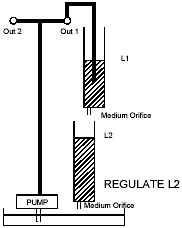
\includegraphics{images/1_relatorio/config_2.png}
    \caption{Sistema de tanques Acoplados}
    \label{fig:sistema_de_tanques_acoplados}
\end{figure}

%\newpage
%\cite{scilab2010}   
 
 
% tem que explicar o que é  sistema dinâmico de tanques acoplados: explicado (copiado do roteiro)
% software SCILAB/Xcos explicado

\end{flushleft}

\newpage

%%%%%%%%%% REFERENCIAL TEÓRICO %%%%%%%

\thispagestyle{main}

\section{REFERENCIAL TEÓRICO}

% \subsection{Controladores PID e Sistemas Dinâmicos de Primeira Ordem}
% %\subsection{Sistemas de Primeira Ordem}\hspace{4ex}

% \hspace{4ex}O controlador PID, na realidade, pode ser visto como sendo uma família de controladores. As 3 ações de controle podem ser combinadas de diferentes maneiras, formando controladores que podem receber diferentes nomes, como: P, PI, PD, PID, conforme as ações de controle são, ou não, utilizadas.

% \begin{enumerate}
%     \item Controle Proporcional (P):
%     \[u(t)=Kpe(t)\] 
%     \[U(S)=KpE(S)\]
%         \begin{itemize}
%             \item O controlador proporcional é um amplificador, com ganho ajustável (K);
%             \item O aumento do ganho K, diminui o erro de regime;
%             \item Em geral, o aumento de K torna o sistema mais oscilatório, podendo instabilizá-lo;
%             \item Melhora o regime e piora o transitório, sendo bastante limitado.
%         \end{itemize}
        
%     \item Controle Proporcional + Integral (PI):
%     \[u(t)=Kp(e(t)+\frac{1}{\tau i}\int_{0}^{t}e(\tau)d\tau)\]
%     \[U(S)=\frac{(KpS+Ki)}{s}E(s)\]
%         \begin{itemize}
%             \item A ação integral do controlador move a variável de controle C(S) baseada na integral no tempo do erro, sendo: \[Ki=\frac{Kp}{\tau i}\], em que: \[\tau i\] é o tempo integrativo, ou tempo de \emph{reset}, com unidade da ordem de minutos;
%             \item Zera o erro de regime, pois aumenta o tipo do sistema em 1 unidade;
%             \item É utilizado quanto tempos resposta transitória aceitável e resposta em regime insatisfatória;
%             \item Adiciona um pólo em p=0 e um zero em \[z=\frac{ki}{kp}=\frac{-1}{\tau i}\]
%             \item Como aumenta a ordem do sistema, temos possibilidade de instabilidade diferente do sistema original. Pode degradar o desempenho do controlador em malha fechada.
%         \end{itemize}
        
%     \item Controle Proporcional + Derivativo (PD):
%         \[u(t)=Kp(e(t)+\tau d\frac{de(t)}{dt})\]
%         \[U(S)=(Kp+KdS)E(S)\]
%         \begin{itemize}
%             \item Sendo: \[Kd=Kp\tau d\] a constante derivativa, dada em minutos.
%             \item Leva em conta a taxa de variaçao do erro;
%             \item É utilizado quando temos resposta em regime aceitável e resposta transitória insatisfatória;
%             \item Adiciona um zero em \[z=\frac{-Kp}{Kd}=\frac{-1}{\tau d}\]
%             \item Introduz um efeito de antecipação no sistema, fazendo com que o mesmo reaja não somente à magnitude do sinal de erro, como também à sua tendência para o instante futuro, iniciando, assim, uma ação corretiva mais cedo;
%             \item A ação derivativa tem a desvantagem de amplificar os sinais de ruído, o que pode causar um efeito de saturação nos atuadores do sistema.
%         \end{itemize}
        
%     \item Controle Proporcional + Integral + Derivativo (PID):
%         \[u(t)=Kp(e(t)+\frac{1}{\tau i}\int_{0}^{t}e(\tau)d(\tau)+\tau d\frac{de(t)}{dt})\]
%         \[U(S)=(Kp+\frac{Ki}{s}+KdS)E(S) => \frac{U(S)}{E(S)}=\frac{KdS^2+KpS+Ki}{S}\]
%         \begin{itemize}
%                     \item É utilizado quando temos resposta transitória e em regime insatisfatórias simultaneamente;
%             \item Adiciona um pólo em p=0 e 2 zeros, que dependem dos parâmetros do controlador.
%         \end{itemize}
        
%     \item Implementação do Controlador PID:
%         \begin{itemize}
%             \item Diferentes equipamentos, de diferentes fabricantes, podem apresentar pequenas variações quanto à implementação do controlador PID. As duas implementações mais comumente utilizadas são: \textbf{Ideal} e \textbf{Paralelo}.
%         \end{itemize}
        
%     \item Modificações das Ações de Controle PID:
%         \begin{itemize}
%             \item Existem também diversas modificações, que poderão ser necessárias em cada implementação, dependendo de características do sistema que estiver sendo controlado, das condições de operações as quais o sistema será submetido e, até mesmo, do equipamento que será utilizado para implementação do controlador.
%         \end{itemize}
        
%         \begin{enumerate}
%             \item Modificação na Ação Derivativa:
%                 \begin{itemize}
%                     \item Filtro da Ação Derivativa
%                         \begin{figure}[h]
%                             \centering
%                             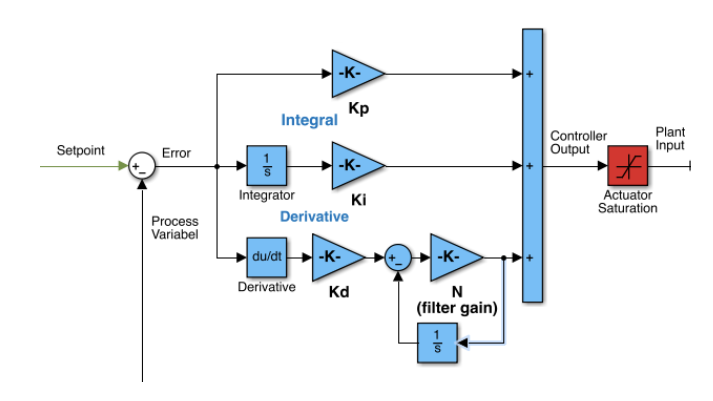
\includegraphics[width=15cm]{images/roteiro a/img ref teorico/filtro_de_acao_derivativa.png}
%                             \caption{Filtro de Ação derivativa}
%                             \label{fig:filtro_de_acao_derivativa}
%                         \end{figure}
%                     \item PI-D
%                         \begin{figure}[h]
%                             \centering
%                             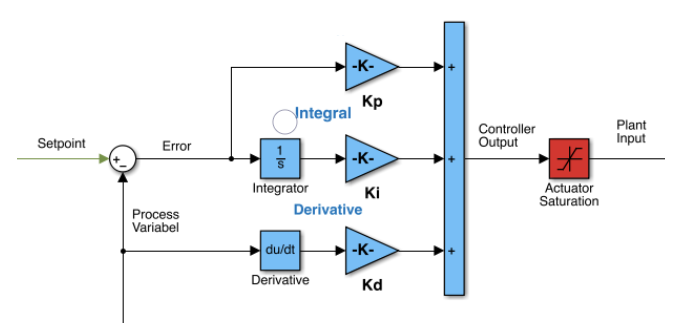
\includegraphics[width=15cm]{images/roteiro a/img ref teorico/pid.png}
%                             \caption{PI-D}
%                             \label{fig:pid}
%                         \end{figure}
%                         \begin{itemize}
%                             \item Objetivo: Não derivar variações bruscas no sinal de referência. 
%                         \end{itemize}
%                         \newpage
%                     \item I-PD
%                          \begin{figure}[h]
%                             \centering
%                             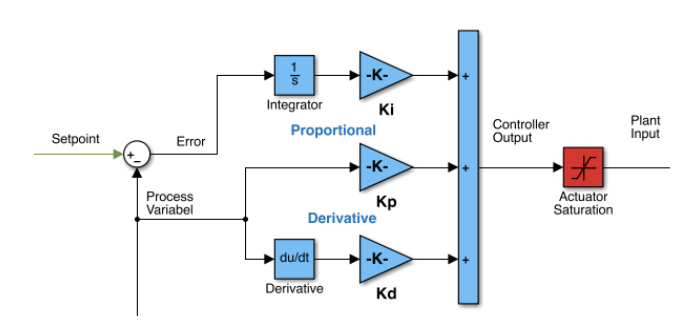
\includegraphics[width=15cm]{images/roteiro a/img ref teorico/ipd.png}
%                             \caption{I-PD}
%                             \label{fig:ipd}
%                         \end{figure}
%                         \begin{itemize}
%                             \item Objetivo: Não derivar, nem amplificar variações bruscas no sinal de referência. 
%                             \\
%                         \end{itemize}
%                 \end{itemize} 
%             \item Modificação na Ação Integrativa:
%                 \begin{itemize}
%                     \item Filtro Anti-Windup (Anti-Reset Windup)
%                 \end{itemize}
%                     \begin{figure}[h]
%                             \centering
%                             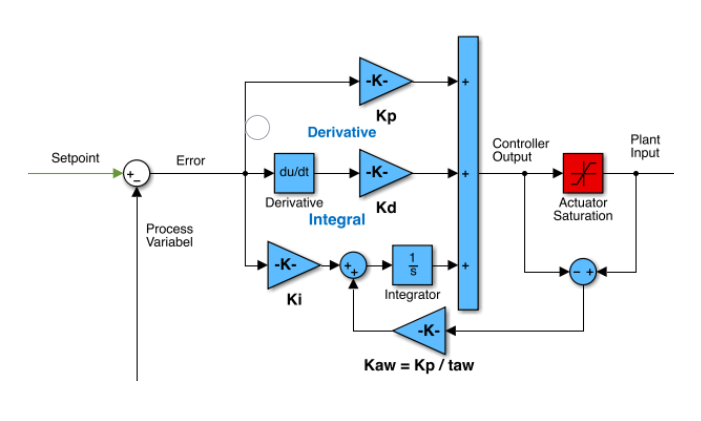
\includegraphics[width=15cm]{images/roteiro a/img ref teorico/filtro_anti_windup.png}
%                             \caption{Filtro Anti-Windup (Anti-Reset Windup)}
%                             \label{fig:filtro_anti_windup}
%                         \end{figure}
%         \end{enumerate}
% \end{enumerate}
\newpage

\subsection{Sistemas de Segunda Ordem}\hspace{4ex}

\subsection{Sistemas de Segurança Instrumentados ou Intertravamentos}\hspace{4ex}

\subsection{Sistemas Dinâmicos na Configuração de Controle em Cascata}\hspace{4ex}

\newpage

%%%%%%%%%% METODOLOGIA %%%%%%%%%%%%%%%

\thispagestyle{main}

\section{METODOLOGIA}\hspace{4ex}
de fato escrever alguma coisa, como foi feita a simulação
\newpage

%%%%%%%%%% RESULTADOS %%%%%%%%%%%%%%%


\newcommand{\labSubFigure}[4]{
% o tipo do sistema 1 ou 2
% tipo do controlador P
% final do arquivo -> #3
% titulo
\ifnum#1=1
    \def \roteiro {roteiro a}
    \def \sistema {sistema tipo 1 }
\fi
\ifnum#1=2
    \def \roteiro {roteiro b}
    \def \sistema {sistema tipo 2 }
\fi
%
\def \controlador{controlador #2}
\def \ganho{#3.pdf}
\def \caminhoImagem{images/\roteiro/\controlador/\ganho}
%
%
\begin{subfigure}[b]{.5\textwidth}
  \centering
  \includegraphics[width=.8\linewidth]{\caminhoImagem}
  \caption{\sistema $#4$}
\end{subfigure}%
}

\thispagestyle{main}

\section{RESULTADOS e DISCUSSÕES}\hspace{4ex}
resultados obtidos do simulador e discutir eles
explicar como essa seção foi dividida



\subsection{Controlador P}\hspace{4ex}

\begin{figure}[h]
\labSubFigure{1}{P}{kp_5}{K_p=5}%1-1
\labSubFigure{2}{P}{kp_10}{K_p=10}%2-1
\labSubFigure{1}{P}{kp_10}{K_p=10}%1-2
\labSubFigure{1}{P}{kp_20}{K_p=20}%1-3
\labSubFigure{2}{P}{kp_20}{K_p=20}%2-2
\labSubFigure{2}{P}{kp_100}{K_p=100}%2-3
\end{figure}

\subsection{Controlador PI}\hspace{4ex}
\begin{figure}
\labSubFigure{1}{PI}{kp_20_ki_0_5}{K_p=20 \quad K_i=0.5}%1-1
\labSubFigure{2}{PI}{kp_20_ki_0_01}{K_p=20 \quad K_i=0.01}%2-1
\labSubFigure{1}{PI}{kp_20_ki_5}{K_p=20 \quad K_i=5}%1-2
\labSubFigure{1}{PI}{kp_20_ki_10}{K_p=20 \quad K_i=10}%1-3
\labSubFigure{2}{PI}{kp_20_ki_0_5}{K_p=20 \quad K_i=0.5 }%2-2
\labSubFigure{2}{PI}{kp_20_ki_0_005}{K_p=20 \quad K_i=0.005}%2-3
\end{figure}



\subsection{Controlador PD}\hspace{4ex}

\begin{figure}
\labSubFigure{1}{PD}{kp_20_ki_0_5}{K_p=20 \quad K_i=0.5}%1-1
\labSubFigure{2}{PD}{kp_20_ki_0_01}{K_p=20 \quad K_i=0.01}%2-1
\labSubFigure{1}{PD}{kp_20_ki_5}{K_p=20 \quad K_i=5}%1-2
\labSubFigure{1}{PD}{kp_20_ki_10}{K_p=20 \quad K_i=10}%1-3
\labSubFigure{2}{PD}{kp_20_ki_0_5}{K_p=20 \quad K_i=0.5 }%2-2
\labSubFigure{2}{PD}{kp_20_ki_0_005}{K_p=20 \quad K_i=0.005}%2-3
\end{figure}

\subsection{Controlador PID}\hspace{4ex}

\subsection{Controlador PID com filtro na ação derivativa}\hspace{4ex}

\subsection{Controlador PID com filtro anti-reset-windup}\hspace{4ex}

\subsection{Sistema de Controle Mestre-Escravo}

\subsubsection{Controlador Mestre P}

\subsubsection{Controlador Mestre PI}

\subsubsection{Controlador Mestre PD}

\subsubsection{Controlador Mestre PID}

\subsubsection{Controlador Mestre PID com filtro na ação derivativa }

\newpage

%%%%%%%%%% CONCLUSÃO %%%%%%%%%%%%%%%

\thispagestyle{main}

\section{CONCLUSÃO}\hspace{4ex}
O que podemos de fato concluir

\newpage

%%%%%%%% REFERÊNCIAS %%%%%%%%%%%%%%%%%

% \section{REFERÊNCIAS BIBLIOGRÁFICAS}

\bibliographystyle{bib/ppgee}
% Referências bibliográficas (geradas automaticamente)
\phantomsection
\addcontentsline{toc}{section}{Referências}
\bibliography{bib/bibliografia}

\appendix

%Apêndice A
\include{apendice}

\end{document}